\chapter{Ondorioak.}


Gure helburua, eguzki-sistemaren doitasun altuko eta epe luzeko integraziorako, Gaussen metodo inplizituaren inplementazio eraginkorra lortzea da. Helburua lortu dugun ala ez galderari erantzuteko, balorazioa bi ikuspegietatik eman behar dela iruditzen zaigu. Batetik, lortutako inplementazioaren aldeko argumentuak azalduz, eraginkorra dela defenditu daiteke. Bestetik, eraginkortasuna,  inplementazioak etorkizunean izan ditzakeen hobekuntzen arabera neurtu beharko litzateke. 

Gakoetako bat, integratu nahi den eguzki-sistemaren ereduaren konplexutasuna da. Eguzki-sistemaren ezagutza gero eta zehatzagoa denez, eredu gero eta konplexuagoak integratuko direla suposatu daiteke. Zentzu honetan, integrazio metodoa problema konplexuen integraziorako eraginkorra izan beharko luke. Edozein kasutan, argi dago, integrazio metodoak  problemaren formulazio matematikoa ez duela mugatu behar eta askatasuna behar dela, ekuazioetan nahi diren efektuak gehitzeko.   

Algoritmoen eraginkortasunaren balorazioa, konputagailu hardware ingurune bati lotuta dago. Ezaguna da, egungo konputagailuen ahalmen handia, konputazio paraleloan oinarritzen dela eta algoritmo eraginkorrak garatzeko, idei berriak aplikatu behar direla. Ausartuko ginateke esaten, Gauss metodo inplizituak, inplementatzeko aukera asko eskaintzen dituenez, egungo idei berri hauek aplikatzeko bidea errazten duela \cite{Dongarra2017}.   


\section*{Eguzki-sistemaren integraziorako inplementazioa.}


Eguzki-sistemaren integraziorako Gauss-en metodo orokorra aplikatu dugula azpimarratu behar dugu. Hori dela-eta, inplementazioa sinplea da eta inplementazioak, metodoaren ezaugarri on guztiak heredatzen ditu. Azken finean, puntu-finkoaren iterazioan oinarritutako IRK inplementazio estandarra aplikatu dugu, formulazio eta geratze irizpide bereziekin. Epe luzeko integrazioetarako, metodoa sinplektikoa izatea garrantzitsua da; IRK metodoaren formulazio estandarrak ez du sinplektikotasuna ziurtatzen, eta horregatik, IRK metodoa aplikatzeko formulazio berria proposatu genuen. Modu berean, geratze irizpide berria inplementazio estandarrarena hobetzeko aplikatu dugu. Beraz, inplementazio berri batek izan ditzakeen konplexutasunak ekidin ditugu. 

Kepler-en fluxuan oinarritutako aldagai aldaketa, ebatzi nahi dugun problemari lotuta dago. Aldagai aldaketa hau, teknika orokor baten aplikazioa da; ekuazio diferentzialetatik zati bat desagertzeko helburuarekin definitutako aldagai aldaketa aplikatzea. Aldagai aldaketa honekin, ekuazio diferentzialetatik alde Kepleriarrari dagokion zatia desagertzea lortzen dugu eta mantso aldatzen den ekuazio diferentzialak lortzen ditugu.  Aldagai berriekiko ekuazio diferentzialak, hiru abantaila ditu. Lehenik, eguzki-sistemaren trunkatze errore nagusiena ezabatu dugunez, integrazioan urrats luzera handiak erabili daitezke. Bigarrenik, integrazioaren urratsaren konputazioaren baturan,
\begin{equation*}
 (\tilde{y}_{n+1}, e_{n+1}) \leftarrow \text{batura konpensatua}(\tilde{y}_n, e_n,\delta_n),
\end{equation*}
$\delta_n$ magnitude txikia du eta beraz, batuketa honetan informazio gutxiago galduko dugu. Gainera, $\delta_n$ doitasun altuan kalkulatzeak abantaila areagotu egiten du. Hirugarrenik, puntu-finkoaren konbergentzia azkarra da.

Eguzki-sistema eredu konplexuetan, Kleperiarrak ez diren indarrak aplika daitezke. Aldagai hauen konbergentzia azkartzeko, Newton sinplifikatuaren iterazioan oinarritutako inplementazioa aplikatzea komeniko da.                  

Gauss metodoa, neurri batean  Splitting eta konposizio metodoen baliokideak dira. 
\begin{align*}
\text{Konposizio metodoa} \ \ &\equiv \ \ \text{Gauss metodoa aldagai aldaketa gabe}.\\
\text{Splitting metodoa}  \ \ &\equiv \ \  \text{Gauss metodoa aldagai aldaketarekin}.
\end{align*}

Splitting metodoekiko antzekotasuna azaltzeko, (\ref{eq:stverlet})~\emph{Störmer-Verlet} Splitting metodoarekin konparatuko dugu. \emph{Störmer-Verlet} metodoa, era honetan aplikatzen da: $h/2$ fluxua aplikatu, perturbazioak kalkulatu eta berriz,  $h/2$ fluxua aplikatu. Gauss metodoan, Kepler-en fluxuan oinarritutako aldagai aldaketa aplikatzen dugunean, gauza bera egiten ari gara: $h/2$ fluxua aurreratu, perturbazioak kalkulatu (aldagai berrietan eta beraz, hobeto kalkulatzen dugu), $h/2$ fluxua aurreratu (\ref{fig:urratsBat}~irudia).

\begin{figure} [h!]
\centerline{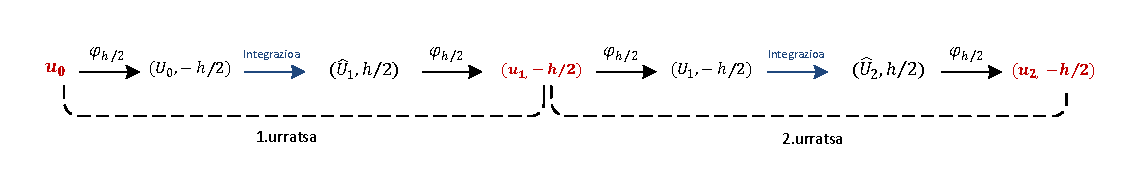
\includegraphics [width=16cm, height=4cm] {urratsBat}}
\caption{\small Gauss metodoan, Kepler-en fluxuan oinarritutako aldagai aldaketa aplikatzen dugunean, urrats baten konputazioa}
\label{fig:urratsBat}
\end{figure} 

Splitting metodoak oso eraginkorrak dira eta eguzki-sistemaren eredu sinplearen integrazioen  esperimentuek, hori erakutsi digute. Baina eredu errealistagoak (gorputz kopurua handitzen delako edota erlatibitate efektua kontutan hartzen delako) integratzeko, Kepler fluxuan oinarritutako Gauss metodoak, Splitting metodoekiko abantailak hauek izango dituela azpimarratuko dugu:  

\begin{enumerate}

\item Ordena altuko metodoak.

Konposizio eta  Splitting metodo optimoenak, $p=10$ ordenakoak dira. Gauss metodoei dagokienez, edozein ordenako metodoak eraiki daitezke. Adibidez, Gaussen $s=16$ ataletako metodoa ($p=32$ ordenako metodoa) eta $80$-biteko doitasuneko koma higikorra aplikatzen baditugu, inplementazioaren zati batzuk $128$-biteko doitasunean kalkulatuz, soluzioaren doitasuna hobetuko dugu.  

\item Paralelizagarria.

Gauss metodoaren $s$-ataletako funtzioen ebaluazioak independenteak dira eta modu paraleloan exekutatu daitezke. Eguzki-sistemaren eredu konplexuagoa kontutan hartzen den neurrian, paralelizazioak abantaila handiagoa suposatuko du. Gauss metodoaren paralelizazio gaitasun hau azpimarratzekoa da, egungo algoritmo azkarren diseinua, kodearen paralelizazioan oinarritzen baita.

\item Hamiltondar orokorrak.

Gauss metodoa, edozein sistema Hamiltondarrari aplika dakioke. Splitting metodoa, ordea, sistema Hamiltondar banagarrietan bakarrik aplika daitezke; eguzki-sistemaren eredu errealistak integratzeko, Hamiltondarraren egitura mantendu behar da eta hainbat indar ez grabitazionalak  gehitzeko, zailtasunak izan ditzakegu. 

\item Malgutasuna.

Splitting metodoen konputazioak, modu trinkoan kalkulatu behar dira, hau da, atalen konputazioak sekuentzialki exekutatzen dira eta metodo esplizituak ez ditu aldaerak onartzen. Gauss metodoaren ekuazio inplizituak ebazteko, ordea, teknika ezberdinak konbina daitezke eta eraginkortasuna hobetzeko aukera asko eskaintzen dizkigu. Adibidez, iterazio gehienak problemaren eredu sinple batekin, doitasun baxuan kalkula daitezke  \cite{Beylkin2014} eta bukaerako iterazio pare bat eredu osoarekin, doitasun altuan. 

\item Birparametrizazioa.

Birparametrizazio, eguzki-sistemaren integrazioetarako tresna baliagarria dela frogatu da \cite{Fukushima2007,Rauch1998} eta Gauss metodoan,  teknika hau zuzenean aplika daiteke. Splitting metodoetan, ordea, birparametrizazioa ezin daiteke erabili eta integrazioetan zailtasunak agertzen direnean (esaterako, planeta baten eszentrikotasuna handitzen denean), orduan integrazioaren tarte batean urratsa txikitu behar dute soluzioaren doitasuna mantentzeko \cite{Laskar2009}.

\end{enumerate}


\section*{Etorkizuneko lanak.}


Etorkizunerako, hobekuntza aukera asko izan ditzake:
\begin{enumerate}
\item Eredu deskonposaketen aplikatutako teknikak.
\item Problema oszilakorren tratamendu aljebraikoan oinarritutako hobekuntza teknikak (metodo prozesatuak, promediatuen teknikak).
\item Kepler fluxuaren hobekuntzak.
\begin{itemize}
\item Kepler-en fluxua: orain iterazio guztietan hasieratik aplikatzen dugu, aurreko iterazioen informazioa erabili gabe. Iterazio berri batean, aurreko iterazioaren egoeratik abiatuta, nahikoa izango da fluxuaren iterazio bakarra egitea.
\item Kepler fluxuaren inplementazioa h txikitarako hobetu daiteke.
\item Paralelizazioa eta bektorizazioa.
\end{itemize}

\item Eredu konplexuak.
Zenbat eta gorputz gehiago izan edo erlatibitate efektua,\dots Era honetako sistemak ditugunean, lehen iterazioetan eredu sinplearekin iteraziok eman daitezke eta azken iterazio pare bat eredu konplexuarekin. 
\end{enumerate} 








